

\begin{frame}{Bearish News for FinTech Lenders Affirm and Klarna}

\begin{center}
    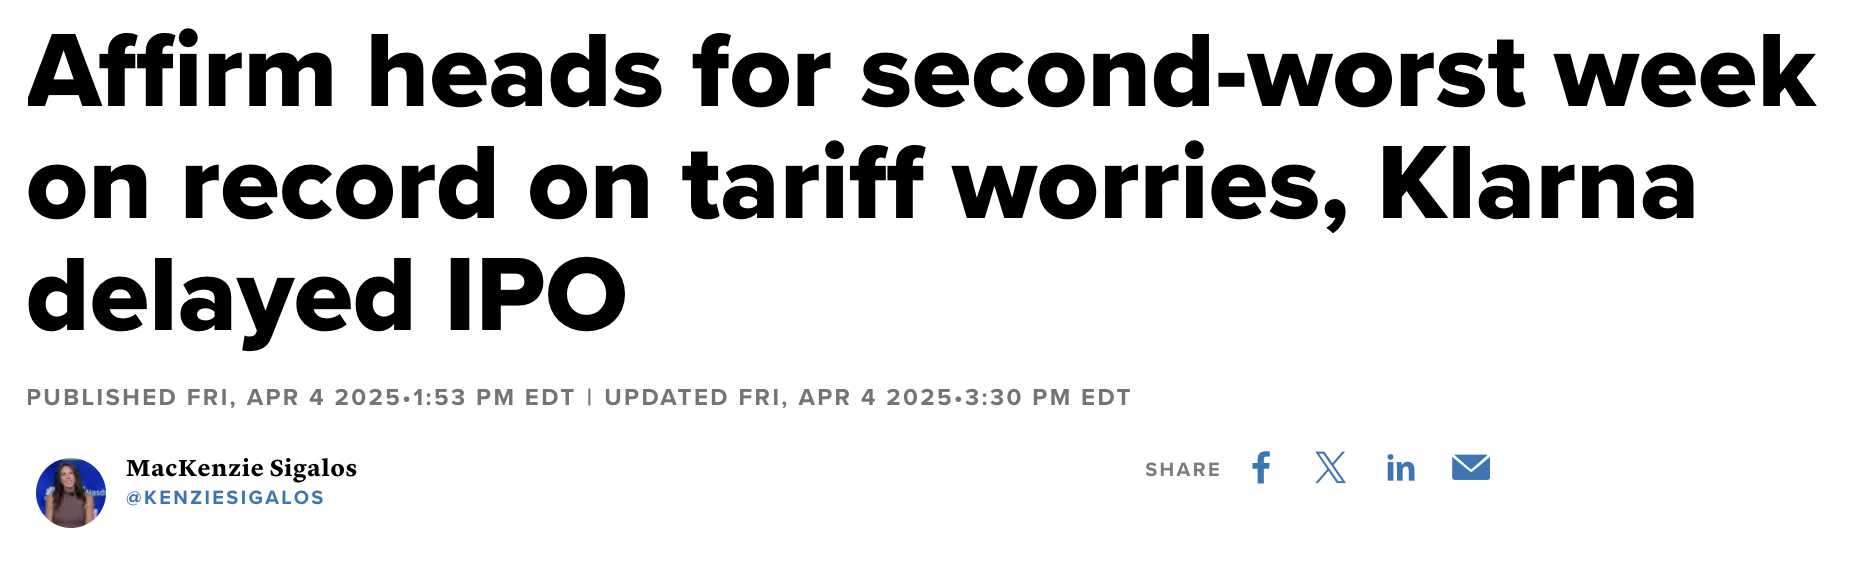
\includegraphics[width = \textwidth]{Crowdfunding/affirm_klarna.png}
\end{center}
    
\end{frame}

\begin{frame}{Fintech Lenders Exposed to Business Cycle Risk}

    \begin{center}
    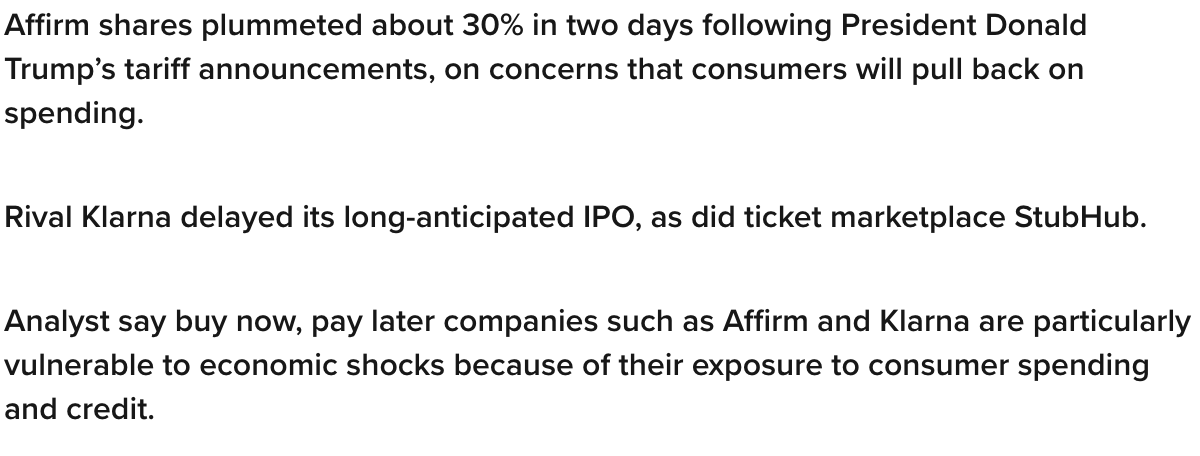
\includegraphics[width = \textwidth]{Crowdfunding/affirm_points.png}
\end{center}
    
    
\end{frame}


\begin{frame}
\frametitle{Retail Lending Sector Pain Points}


What are the pain points that crowdfunding companies try to solve? \\
\smallskip 
\textbf{For Fundraisers (Borrowers / Issuers):}
\begin{itemize}
    \item \textbf{Access to Capital} -- bypasses traditional gatekeepers (banks and VCs are inaccessible for early-stage or non-traditional ventures.)
    \item \textbf{Speed \& Simplicity} -- fast online application and launch than with traditional banks and VCs.
    \item \textbf{Market Validation} -- test product/idea demand from early supporters, not possible with banks or VCs.
    \item \textbf{Lower Fundraising Costs} -- fewer legal/admin burdens than banks.
    \item \textbf{Audience Engagement} -- build community and future customers, not possible with banks or VCs.
\end{itemize}



	
\end{frame} 
%----------------------------------------------------  




%------------------------------------------------

\begin{frame}
\frametitle{Retail Lending Sector Pain Points}


What are the pain points that crowdfunding companies try to solve? \\
\smallskip 
\textbf{For Funders (Investors / Backers):}
\begin{itemize}
    \item \textbf{Access to New Opportunities} -- invest in startups, real estate, or social ventures that were traditionally reserved for accredited investors or institutions.
    \item \textbf{Diversification} -- small minimums across many projects
    \item \textbf{Emotional/Social Return of Investment} -- support causes or innovations they believe in
\end{itemize}


	
\end{frame} 
%----------------------------------------------------  





%------------------------------------------------

\begin{frame}
\frametitle{Robot Advisors Basics}
\vspace{-2mm}
Economies of Scale and Customer Acquisition
\begin{itemize}
  \item Robo-advice started as a disruptive niche fintech product.
  \item Now consolidated around a few large players, mostly owned by incumbent financial institutions.
  \item Independent fintech robo-advisors are rare survivors.
  \item \textbf{Key challenges:}
  \begin{itemize}
    \item Low fees
    \item High customer acquisition costs
    \item Low barriers to entry
    \item Intense competition
  \end{itemize}
  \item Technology alone is not a sustainable competitive advantage — it can be copied or acquired by fast-followers.
  \item \textbf{Biggest barrier to entry:} Access to customers and \textbf{trust} of those customers 
\end{itemize}



\end{frame} 
%----------------------------------------------------  





%------------------------------------------------

\begin{frame}
\frametitle{Robot Advisors Basics}

\vspace{-2mm}
Wealth Management is a \$100 trillion Industry

\begin{itemize}
    \item Wealth mgt covers many activities: financial planning, portfolio management, \& back-office operations.
\end{itemize}

\smallskip 

Digital wealth management is changing how financial advisors serve customers


\begin{itemize}
    \item Technologies such as cloud computing, data science, APIs, cryptography, blockchain, and artificial intelligence lower costs, increase productivity, and improve the customer experience.

    \item Fintechs in the business-to-consumer (B2C) space provide investing algorithms and mobile apps, analytics, customer onboarding, relationship management, risk management, cybersecurity tools, and regtech.

    \item In theory, the result is better service, lower fees, and greater transparency.

\end{itemize}

\end{frame} 
%----------------------------------------------------  








%------------------------------------------------

\begin{frame}
\frametitle{Robot Advisors Basics}



\vspace{-2mm}
From Investing to Financial Planning
\begin{itemize}
  \item The original robo-advisors were fully automated to minimize costs with no human interaction.

  \item Most now offer a hybrid service, with access to a salesperson or registered financial advisor for a fee.

  \item Robo-advisors have been expanding into: (1) brokerage; (2) financial planning; (3) personal finance; (4) tax reporting, and even (5) banking
\end{itemize}




\end{frame} 
%----------------------------------------------------  




%------------------------------------------------

\begin{frame}
\frametitle{The Wealth Management Industry}


\vspace{-2mm}
\begin{itemize}
    \item Fintechs leverage technology to provide retail investors the same sophisticated, personalized services as high net worth investors.
    \begin{itemize}
        \item Did not use to be economically feasible to offer a retail customer this level of service due to low AUM and cost of the financial advisor.
    \end{itemize}

    \item \textbf{Digital wealth management} leverages technology to automate and improve the customer experience.
    \begin{itemize}
        \item Automating standard, repetitive tasks to lower costs, increase productivity, and offer more value to investors
        \item Use cases:
        \begin{itemize}
            \item Portfolio construction and management
            \item Customer relationship management (CRM)
            \item Know-your-customer (KYC)
            \item Anti-money laundering (AML)
            \item Cybersecurity
            \item Regulatory compliance
        \end{itemize}
    \end{itemize}
\end{itemize}



\end{frame} 
%----------------------------------------------------  



%------------------------------------------------

\begin{frame}
\frametitle{How Have Incumbents Responded to Robot Advisors}


\vspace{-2mm}
\begin{itemize}
    \item Largest mutual fund companies and broker-dealers have been fast-followers, developing a robo in-house or licensing software from a start-up.
    \begin{itemize}
        \item 2013 Vanguard Group; 2014 Charles Schwab; 2016 BoA Merrill Lynch, Capital One, E*Trade, Fidelity, and TD Ameritrade
    \end{itemize}
    \item Following strategy of Harvard’s Clayton Christensen:
    \begin{itemize}
        \item Don't overreact; continue to serve profitable customers
        \item Invest to improve primary product (sustaining innovations)
        \item Launch a low-cost, no-frills service of their own
    \end{itemize}
    \item Examples: 
    \begin{itemize}
        \item White labeled robo-advisor software (e.g., Betterment for Advisors)
        \item Licensed robo-advisor software from SigFig (e.g., UBS, JPMorgan, NY Life, Wells Fargo, Santander)
        \item Acquired a robo-advisor (BlackRock → FutureAdvisor)
    \end{itemize}
\end{itemize}

\end{frame}




%------------------------------------------------

\begin{frame}
\frametitle{The Wealth Management Industry}


\vspace{-2mm}
\begin{itemize}
    \item At \$100 trillion of AUM, the wealth management industry is massive and profitable.
    \begin{itemize}
        \item Job titles include: (1) Financial advisor, financial planner, relationship manager, salesperson; (2) Portfolio manager, trader, research analyst, private banker (3) Private equity specialist, risk manager, and more…
    \end{itemize}
 

    \item There are two sides to this industry:

    \begin{itemize}
        \item \textbf{Wholesale}: dominated by institutional investors: asset mgt firms, pension funds, mutual funds, insurance companies, and banks.
        

        \item \textbf{Retail}: individual investors who are advised by financial advisors, registered investment advisors (RIAs), financial planners, wealth managers, and investment counselors.
        \begin{itemize}
            \item High net worth (HNW) are \$1 million+, ultra-high net worth (UHNW) are \$30 million+.
        \end{itemize}
    \end{itemize}
\end{itemize}




\end{frame} 
%----------------------------------------------------  



%------------------------------------------------

\begin{frame}
\frametitle{The Wealth Management Industry}


\vspace{-2mm}
\begin{itemize}
    \item To understand the opportunities and pain points, let's look at the wealth management value chain:
    \begin{itemize}
        \item \textbf{Acquire customers and investments}
        \item \textbf{Portfolio management}
        \item \textbf{Operations (back-office)}
    \end{itemize}
\end{itemize}


\vspace{-6mm}
%-----------------------------------------------
\begin{figure}[H]
    \resizebox{5.6in}{1.2in}{%
    %\resizebox{\textwidth}{!}{%
    
\includegraphics[]{figures/WealthManagement_ValueChain.png}
    } %end of resizebox
%-----------------------------------------------
% Figure setting: caption and label
%-----------------------------------------------
%\caption{Insurtech Performance First Year Post-IPO}
%\label{fig:ModelIntuition_Graphs}
\end{figure}
%-----------------------------------------------
\vspace{-2mm}


\begin{itemize}
    \item \textbf{Know your customer (KYC):}
    \begin{itemize}
        \item Verifying the identity of a client
        \item Evaluating their financial knowledge and risk tolerance
        \item Establishing what investments are suitable
    \end{itemize} 
\end{itemize}



\end{frame} 
%----------------------------------------------------  


%------------------------------------------------

\begin{frame}
\frametitle{The Wealth Management Industry}


\vspace{-2mm}
The Technology-Enabled \textit{eAdvisor}
\begin{itemize}
    \item A traditional financial advisor can manage 200 clients. 
    \begin{itemize}
        \item If they charge 2.0\% of Assets Under Management (AUM) and the average customer has \$100,000, the advisor collects \$400,000 before expenses.
        \item It did not make sense to manage customers with only \$10,000 to invest.
    \end{itemize}
    \item Research by Fidelity finds that eAdvisors can manage more clients with 42\% higher AUM.
    \begin{itemize}
        \item eAdvisors are younger, use social media, video conferencing, and automated email alerts to stay in touch.
        \item They offer e-signature options and provide electronic delivery of statements and reports.
        \item They use data aggregation tools to provide the total picture of clients’ assets and liabilities.
    \end{itemize}
\end{itemize}



\end{frame} 
%----------------------------------------------------  




%------------------------------------------------

\begin{frame}
\frametitle{The Wealth Management Industry}



\vspace{-2mm}
Digital Customer Onboarding
\begin{itemize}
    \item Customer relationship management (CRM) is a key success factor in wealth management.
    \begin{itemize}
        \item It is also a pain point due to manual workflows, administration, and legacy IT systems.
        \item Customer onboarding with KYC and AML is a time-consuming, paper-based process.
    \end{itemize}
    \item Robo-advisors such as Nest Wealth have found product-market fit in the B2B space by licensing their customer onboarding and CRM software tools to financial advisors.
\end{itemize}


\vspace{-6mm}
%-----------------------------------------------
\begin{figure}[H]
    \resizebox{5.6in}{1in}{%
    %\resizebox{\textwidth}{!}{%
    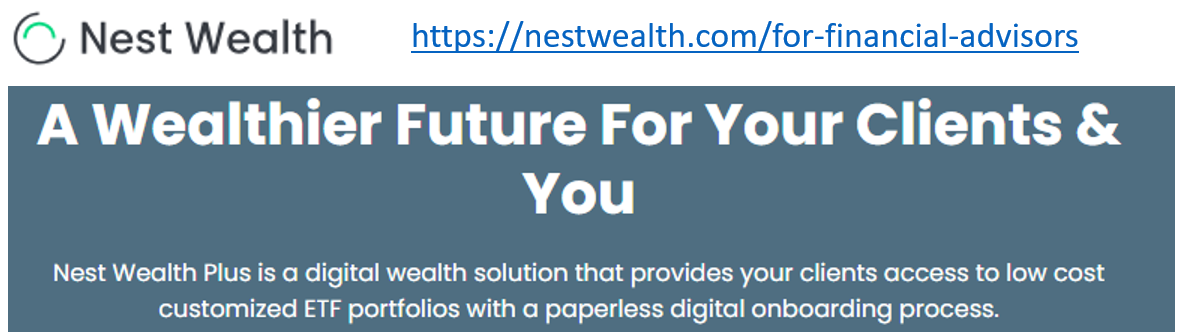
\includegraphics[]{figures/NestWealth.png}
    } %end of resizebox
%-----------------------------------------------
% Figure setting: caption and label
%-----------------------------------------------
%\caption{Insurtech Performance First Year Post-IPO}
%\label{fig:ModelIntuition_Graphs}
\end{figure}
%-----------------------------------------------
\vspace{-2mm}


\end{frame} 
%----------------------------------------------------  


\begin{frame}
\frametitle{How Crowdfunding Portals Make Money}


Crowdfunding portals have same expenses as a traditional financial intermediary:
\begin{itemize}
    \item Sales and marketing expenses (cost of customer acquisition)
    \item Technology costs
    \item Research and development
    \item Salaries, benefits, and employee compensation
    \item General and administrative expenses (e.g., overhead)
    \item Distribution, processing, and servicing costs
    \item Corporate taxes
    \item Funding costs for balance sheet lenders
    \item Write-downs on non-performing loans for balance sheet lenders
\end{itemize}



\end{frame} 
%----------------------------------------------------  


\begin{frame}
\frametitle{Conclusion}


Crowdfunding provides a new business model for fundraising that directly matches borrowers and lenders online, outside of traditional finance.

\medskip 

Crowdfunding is more successful for equity, donations, and rewards for good products (like pepwatch) and art projects that are not served well by traditional finance. 

\medskip 

Crowdfunding continues to grow but very slowly recently. 

\medskip 

However, crowdfunding struggles to compete with traditional finance in customers that have already been served because crowdfunding does not offer a much better method: 
\begin{itemize}
    \item reducing (information asymmetry-induced) adverse selection problem
    \begin{itemize}
        \item Credit bureau data is somewhat mature. Alternative data does not provide comprehensive advantages. 
    \end{itemize}
    \item reducing (information asymmetry-induced) moral hazard problem
    \begin{itemize}
        \item Traditional finance institutions are still good at monitoring
    \end{itemize}
\end{itemize}




\end{frame} 
%----------------------------------------------------  
